% Sketch output, version 0.3 (build 7d, Sun Mar 20 14:11:05 2016)
% Output language: PGF/TikZ,LaTeX
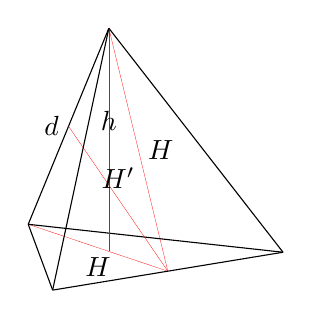
\begin{tikzpicture}[line join=round]
\draw[line width=.1pt,draw=red](-2.055,-1.034)--(-.282,-1.63);
\draw(-2.055,-1.034)--(-1.745,-1.87);
\draw(-1.031,1.456)--(-2.055,-1.034);
\draw(-2.055,-1.034)--(1.181,-1.389);
\draw[line width=.1pt,draw=red](-.282,-1.63)--(-1.543,.211);
\draw[line width=.1pt,draw=red](-1.031,1.456)--(-1.031,-1.378);
\draw(1.181,-1.389)--(-1.031,1.456);
\draw(1.181,-1.389)--(-1.745,-1.87);
\draw(-1.745,-1.87)--(-1.031,1.456);
\draw[line width=.1pt,draw=red](-1.031,1.456)--(-.282,-1.63);
\node[below] at (-1.169,-1.332) {$H$};\node[right] at (-.657,-.087) {$H$};\node[above] at (-1.031,.039) {$h$};\node[above] at (-.913,-.709) {$H'$};\node[left] at (-1.543,.211) {$d$};\end{tikzpicture}% End sketch output
